% 原书 p.6–p.10（PDF p.14–p.18）
% >>> p014
\section{近复结构（Almost Complex Structure）}

\begin{keytakeaways}
\begin{itemize}
  \item 几何图像：近复结构是在每个切空间上「逐点」模仿乘以 $\sqrt{-1}$ 的线性算子族 $J$，
        它把奇数维的复结构条件降格为逐点的代数条件 $J_p^2=-\mathbf{1}$。
  \item 数学工具：Nijenhuis 张量 $N_J$、Newlander--Nirenberg 定理（可积性判据）、
        以及由辛形式与 Riemann 度量构造 $J$ 的极分解技巧。
  \item 本节结论：任何辛结构都诱导 $\omega$-相容的近复结构（命题 1.3.1），
        从而任何辛流形都是近复流形；反之近复流形未必辛（例 1.3.1 前的讨论）。
        对二维闭曲面，一切近复结构自动可积（例 1.3.1）。
  \item 结构图像：图 1.1 给出「近复 $\supset$ 辛、复」「复 $\supset$ Kähler $\subset$ 辛」的严格包含关系；
        三者的交（Kähler）才是复几何与辛几何的共同地带。
\end{itemize}
\end{keytakeaways}

回忆复流形 $M$（复维数 $n$）是局部以 $\C^n$ 的开子集为模型的流形，其转移映射全都是全纯的，
意即它们与乘以 $\sqrt{-1}$ 的运算交换。当然，我们可以把 $M$ 看作实维数 $2n$ 的实流形：
把复坐标卡 $(U,z)$ 形式地换为实坐标卡 $(U,x,y)$，其中 $x=(x_1,\cdots,x_n)$ 与
$y=(y_1,\cdots,y_n)$ 来自 $z_i=x_i+\sqrt{-1}\,y_i$。近复结构定义在偶数维流形上，
它模仿复流形的全纯条件，但只逐点地定义在每个切空间上。

\begin{wdefn}{1.3.1}
实偶数维流形 $M$ 上的\textbf{近复结构}（almost complex structure）是切空间上的一族光滑
$\R$-线性映射 $J_p:T_pM\to T_pM$，使得对任意 $p\in M$ 都有 $J_p^2=-\mathbf{1}$。
\end{wdefn}

\begin{wrem}{1.3.1}
任何复结构都诱导一个近复结构。事实上，给定复流形 $M$，对任意 $p\in M$ 我们可在局部坐标下
把 $T_pM$ 写成
\[
  T_pM=\mathrm{span}\left\langle
  \frac{\partial}{\partial x_1},\cdots,\frac{\partial}{\partial x_n},
  \frac{\partial}{\partial y_1},\cdots,\frac{\partial}{\partial y_n}\right\rangle .
\]
然后定义 $J_p$ 为
$J_p\left(\dfrac{\partial}{\partial x_i}\right)=\dfrac{\partial}{\partial y_i}$，
$J_p\left(\dfrac{\partial}{\partial y_i}\right)=-\dfrac{\partial}{\partial x_i}$，
并在整个 $T_pM$ 上 $\R$-线性地延拓。于是 $J_p^2=-\mathbf{1}$。
\end{wrem}

为了判别一个近复结构是否由如注 1.3.1 中的复结构所诱导或实现（此时称该近复结构\textbf{可积}），
我们通常应用如下判别准则。在此之前，先引入一个术语：对 $M$ 上的任意向量场 $X,Y$，定义
\textbf{Nijenhuis 张量}（更一般的定义称为 [87] 中的 Frölicher--Nijenhuis 括号）为
\begin{equation}
  N_J(X,Y):=[JX,JY]-J[X,JY]-J[JX,Y]-[X,Y] .
  \tag{1.6}
\end{equation}

\begin{wthm}{1.3.1}（Newlander--Nirenberg\textsuperscript{167}）
$M$ 上的一个近复结构 $J$ 可积，当且仅当由 (1.6) 定义的 Nijenhuis 张量 $N_J$ 满足 $N_J\equiv0$。
\end{wthm}
% [Tutor Note: 易错符号——(1.6) 是文献中最常见的 Nijenhuis 张量定义（例如 [87]、Kobayashi–Nomizu
% 的约定），其符号与「先取 $[JX,Y]$ 还是 $[X,JY]$」以及整体正负号有关：另一族文献写作
% $N_J(X,Y)=[JX,JY]-J[JX,Y]-J[X,JY]+[X,Y]$。两种写法只差 $N_J$ 的整体负号，但「$N_J\equiv0$」
% 这一判据不受影响。需注意 $N_J$ 是张量（不是微分算子）：尽管定义中用到向量场的括号，
% $N_J(fX,Y)=fN_J(X,Y)$ 仍成立，故它逐点取值。]

% >>> p015
有一个让定理 1.3.1 容易应用的漂亮情形：任何闭曲面。

\begin{wexam}{1.3.1}
回忆 $\Sigma_g$ 表示亏格 $g$ 的闭可定向曲面。设 $J$ 为 $\Sigma_g$ 上的近复结构，则 $N_J\equiv0$。
由定理 1.3.1，$\Sigma_g$ 上的任何近复结构都是可积的！

为证明 $N_J$ 的零化结论，我们注意到：对 $\Sigma_g$ 上的任意向量场 $X$，向量场 $X$ 与 $JX$
总是 $\R$-线性无关的。事实上，若对某个实 $\lambda\neq0$ 有 $X=\lambda JX$，则
$JX=\lambda J^2X=-\lambda X$，这说明 $X=\lambda JX=-\lambda^2X$。因此 $(1+\lambda^2)X=0$，矛盾。
从而只需在向量场 $X$ 与 $JX$ 上验证 $N_J\equiv0$：
\[
  \begin{aligned}
    N_J(X,JX)&=[JX,J(JX)]-J[X,J(JX)]-J[JX,JX]-[X,JX]\\
             &=[JX,-X]-J[X,-X]-0-[X,JX]\\
             &=[JX,-X]-[X,JX]=0 .
  \end{aligned}
\]
至此完成了验证。注意我们尚未确认 $\Sigma_g$ 上总存在近复结构（参见命题 1.3.1）。\hfill$//$
\end{wexam}
% [Tutor Note: 这里省略的实质是「在二维情形 $N_J$ 的四个项两两抵消」：$J(JX)=-X$ 使第 1、2 项化为
% $[JX,-X]$ 与 $-J[X,-X]$，而 $[JX,JX]=0$ 消去第 3 项；最后 $[JX,-X]=-[X,JX]$ 归零。
% 更一般地，$N_J$ 在复维数 1 的流形上恒为零，故二维时近复结构必可积（这是 Newlander–Nirenberg
% 定理的最低维特例，其证明不需任何分析）。注意 $X$ 与 $JX$ 线性无关只用到 $J^2=-\mathbf{1}$，
% 与 $M$ 的拓扑无关。]

由于例 1.3.1，当复结构在其中起作用时，闭曲面 $\Sigma_g$ 也称为 \textbf{Riemann 曲面}。
$\Sigma_g$ 上的任何复结构通常记作 $j$。

\begin{wexer}{1.3.1}
$S^6$ 上存在一个不可积的近复结构。（提示：考虑单位纯虚 Cayley 数构成的空间。）
\end{wexer}

迄今为止，我们已经遇到了三种几何结构：辛结构、复结构和近复结构。它们之间的关系如下所述。

图 1.1 中的所有包含关系都是严格的。例如，存在不是辛流形的复流形。标准的反例是一个
\textbf{Calabi--Eckmann 流形} [37]。具体地，对任意 $n\in\N_{\ge1}$，很容易在
$S^1\times S^{2n+1}$ 上赋予一个复结构。然而，由练习 1.1.1，它不允许任何辛结构。除了复结构集合
与近复结构集合之间的包含关系（由注 1.3.1 确认）之外，图 1.1 中的关系还表明：任何辛流形都应当
允许一个近复结构，这一点在下面的结果中被正式陈述。

% >>> p016
\begin{figure}[htbp]
  \centering
  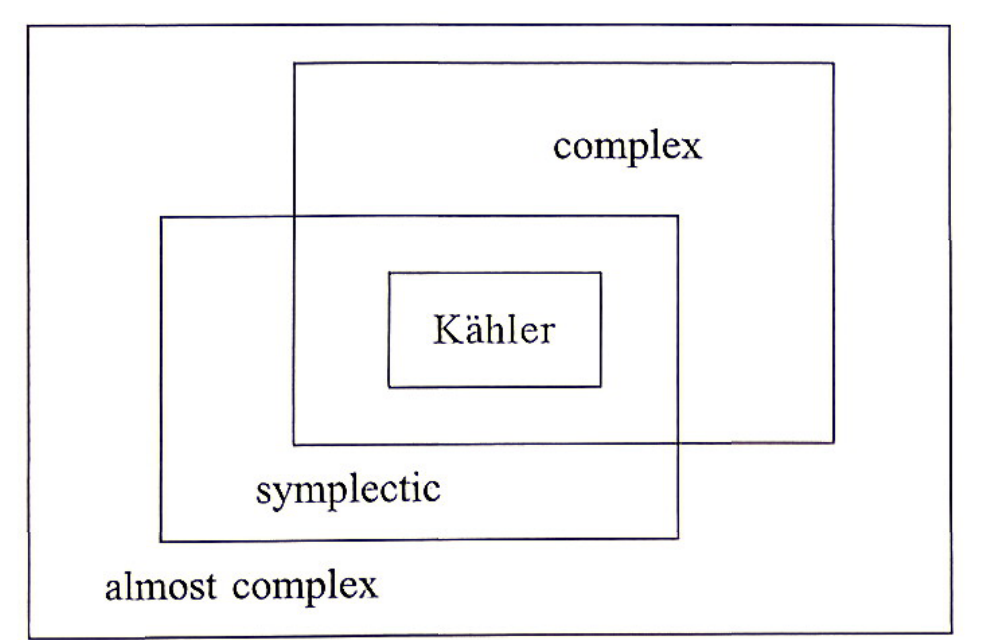
\includegraphics[width=0.66\linewidth]{figures/fig_p016_1.png}
  \caption*{图 1.1\quad 不同几何结构之间的关系（原书 p.8, Figure 1.1；PDF p.16）}
\end{figure}

\begin{wprop}{1.3.1}
任何辛结构都诱导一个近复结构。
\end{wprop}

\begin{wproof}
记底层的辛流形为 $(M,\omega)$，并在 $M$ 上固定一个 Riemann 度量 $g$。由于 $g$ 与 $\omega$
都是非退化的，取 $T_pM$ 的一组基之后，我们便得到 $T_pM$ 上的一个线性同构，记作 $A$。
具体地，对任意 $v,w\in T_pM$，有
\[
  g_p(Av,w)=\omega_p(v,w).
\]
此处我们断言 $A$ 是斜对称的。事实上，一方面
$\omega_p(v,w)=g_p(Av,w)=g_p(v,A^{\mathrm T}w)=g_p(A^{\mathrm T}w,v)$；另一方面
$\omega_p(w,v)=g_p(Aw,v)$。合起来，我们得到
\[
  g_p(A^{\mathrm T}w,v)=-g_p(Aw,v)=g_p(-Aw,v)=g_p(v,-Aw),
\]
这蕴涵 $A^{\mathrm T}=-A$。

接着考虑 $AA^{\mathrm T}$，它是一个对称且实正定的矩阵。定义
$J_p:=(\sqrt{AA^{\mathrm T}})^{-1}\cdot A$。于是
\[
  \begin{aligned}
    J_p^2&=\left(\sqrt{AA^{\mathrm T}}\right)^{-1}\cdot A
          \cdot\left(\sqrt{AA^{\mathrm T}}\right)^{-1}\cdot A\\
         &=\left(AA^{\mathrm T}\right)^{-1}\cdot A\cdot A
          =-\left(AA^{\mathrm T}\right)^{-1}\cdot\left(AA^{\mathrm T}\right)
          =-\mathbf{1}.
  \end{aligned}
\]
因此证明完成。
\end{wproof}
% [Tutor Note: 上述计算隐含了两点：(1) $\sqrt{AA^{\mathrm T}}$ 是 $AA^{\mathrm T}$ 的多项式，
% 因而与 $A$ 交换；(2) 由 $A^{\mathrm T}=-A$ 得 $AA^{\mathrm T}=-A^2$，故
% $A^2=-\left(\sqrt{AA^{\mathrm T}}\right)^2$。这两点合起来才给出
% $\left(\sqrt{AA^{\mathrm T}}\right)^{-1}A\cdot\left(\sqrt{AA^{\mathrm T}}\right)^{-1}A
% =(AA^{\mathrm T})^{-1}A^2=-\mathbf{1}$。初学者常误以为 $\sqrt{AA^{\mathrm T}}$ 与 $A$ 可
% 无条件交换，务必先验证 $AA^{\mathrm T}$ 与 $A$ 可交换。]

\begin{wrem}{1.3.2}
我们要强调：命题 1.3.1 的证明没有用到定义 1.1.1 中的条件 (ii) $\dd\omega=0$。因此，由该证明
所得到的任何诱导几何结构，自然只能反映局部性质。
\end{wrem}

关于命题 1.3.1 所构造的近复结构 $J$，有一个基本观察：所得的 $J$ 满足如下两条性质
\begin{equation}
  \text{(i) }\ \omega(Jv,Jw)=\omega(v,w)
  \qquad\text{以及}\qquad
  \text{(ii) }\ \omega(v,Jv)>0
  \tag{1.7}
\end{equation}
其中 $v,w$ 为任意非零向量。下面我们把验证 (i) 与 (ii) 的细节补全。对 (i)，我们有如下计算：
\[
  \begin{aligned}
    \omega(Jv,Jw)&=\omega\left(\left(\sqrt{AA^{\mathrm T}}\right)^{-1}Av,
      \left(\sqrt{AA^{\mathrm T}}\right)^{-1}Aw\right)\\
    &=\omega\left(A\left(\sqrt{AA^{\mathrm T}}\right)^{-1}v,
      \left(\sqrt{AA^{\mathrm T}}\right)^{-1}Aw\right)\\
    &=g\left(-\left(\sqrt{AA^{\mathrm T}}\right)^{-1}v,
      \left(\sqrt{AA^{\mathrm T}}\right)^{-1}Aw\right)\\
% >>> p017
    &=g\left(-v,\left(\sqrt{AA^{\mathrm T}}\right)
      \left(\sqrt{AA^{\mathrm T}}\right)^{-1}Aw\right)\\
    &=g(Aw,-v)=\omega(v,w).
  \end{aligned}
\]
% [Tutor Note: 原文疑误——上式中第 3 行 $g$ 的第一个自变量应为
% $-\left(\sqrt{AA^{\mathrm T}}\right)v$（而非 $-\left(\sqrt{AA^{\mathrm T}}\right)^{-1}v$）。
% 核对方式：由 $\omega(x,y)=g(Ax,y)$ 与
% $A^2=-\left(\sqrt{AA^{\mathrm T}}\right)^2$ 得
% $\omega\left(A\left(\sqrt{AA^{\mathrm T}}\right)^{-1}v,\cdot\right)
% =g\left(-\left(\sqrt{AA^{\mathrm T}}\right)v,\cdot\right)$；
% 再由 $g$ 的对称性与 $\left(\sqrt{AA^{\mathrm T}}\right)\left(\sqrt{AA^{\mathrm T}}\right)^{-1}
% =\mathbf{1}$ 才能得到第 4 行的 $g(-v,Aw)$。按原文写法则最后一行不成立（一般
% $A^{-1}\neq-A$）。译文保留原文写法，详见 review_ch01.md。]

对 (ii)，我们有如下计算，
\[
  \begin{aligned}
    \omega(v,Jv)&=\omega\left(v,\left(\sqrt{AA^{\mathrm T}}\right)^{-1}Av\right)\\
    &=\omega\left(-A\left(\sqrt{AA^{\mathrm T}}\right)^{-1}v,v\right)\\
    &=g\left(\sqrt{AA^{\mathrm T}}\,v,v\right),
  \end{aligned}
\]
只要 $v$ 非零它便是正的。

与上述类似的验证还表明：任何满足 (1.7) 中条件 (i) 与 (ii)（相对于给定的辛结构 $\omega$）的
近复结构 $J$，都反过来帮我们造出一个 Riemann 度量，记作 $g_J$。具体地，
\begin{equation}
  g_J(v,w):=\omega(v,Jw)
  \tag{1.8}
\end{equation}
其中 $v,w$ 任意。此时 (1.7) 中的条件 (i) 保证 $g_J$ 的对称性，而 (1.7) 中的条件 (ii) 保证
$g_J$ 的非退化性。

\begin{wrem}{1.3.3}
我们可以把上面三种结构 $g,\omega,J$ 放在一起玩：命题 1.3.1 开头从固定的 $g$ 出发构造出 $J$，
再为这个 $J$ 构造度量 $g_J$。回忆 $J=(\sqrt{AA^{\mathrm T}})^{-1}A$，其中 $g(Av,w)=\omega(v,w)$。
则按 (1.8)，$g_J(v,w)=\omega(v,(\sqrt{AA^{\mathrm T}})^{-1}Aw)$；而
$g(v,w)=\omega(A^{-1}v,w)$。因此一般而言 $g$ 与 $g_J$ 并不相同（换言之，$g_J$ 并不能还原出
一开始所用的 $g$）。
\end{wrem}
% [Tutor Note: 这里 $g(v,w)=\omega(A^{-1}v,w)$ 由 $g(Av,w)=\omega(v,w)$ 令 $v\mapsto A^{-1}v$
% 得到。最后一句「$g_J$ 不能还原 $g$」是很有用的提醒：极分解 $A=P\cdot O$ 中 $P=\sqrt{AA^{\mathrm T}}$
% 与 $O=P^{-1}A$ 分别携带度量的「长度」信息与「复结构」信息，而 $J=O$ 只保留了 $O$；
% 等价地，$(\omega,g,J)$ 三者中任意两个相容的结构决定第三个，但此处 $J$ 是由 $g$ 造出的，
% 并不保证 $g_J=g$。]

以下定义概括了 (1.7) 中的各项条件。

\begin{wdefn}{1.3.2}
给定辛流形 $(M,\omega)$，若近复结构 $J$ 同时满足 (1.7) 中的两条条件，则称 $J$ 是
$\omega$-\textbf{相容的}（$\omega$-compatible）；若 $J$ 只满足 (1.7) 中的条件 (ii)，则称 $J$
是 $\omega$-\textbf{驯顺的}（$\omega$-tame）。
\end{wdefn}

根据定义 1.3.2 及其上方的观察，命题 1.3.1 实际上证明了：任何辛结构 $\omega$ 都诱导一个
$\omega$-相容的近复结构。

\begin{wrem}{1.3.4}
有时人们更愿意使用 $\omega$-驯顺的近复结构，因为「$\omega$-驯顺」是一个开条件，对小的扰动
具有灵活性。
\end{wrem}

给定辛流形 $(M,\omega)$，用 $\mathcal{J}(M,\omega)$ 记 $M$ 上所有 $\omega$-相容近复结构构成的集合。
于是下面的练习揭示了 $\mathcal{J}(M,\omega)$ 的拓扑的一个基本性质。

\begin{wexer}{1.3.2}
对任意辛流形 $(M,\omega)$，证明：所有 $\omega$-相容近复结构的集合 $\mathcal{J}(M,\omega)$
是道路连通的。
\end{wexer}

下面这个事实是 Gromov 的一个著名结果，它大大加强了练习 1.3.2 的结论。其引人入胜的证明可在
[153] 中的命题 2.5.13 找到。

% >>> p018
\whead{事实}{1.3.1}（Gromov）\quad 作为拓扑空间，$\mathcal{J}(M,\omega)$ 是可缩的。

后面我们将看到，在辛几何中，把近复结构变化（到某个偏好的近复结构）并证明某个数据在这种形变下
不变，是一项重要的技术。
% [Tutor Note: 「$\mathcal{J}(M,\omega)$ 可缩」比「道路连通」强得多：有了可缩性，任何两条相容近复结构
% 之间可以选取「典范的」（同伦意义下唯一）道路，这正是 Gromov–Witten 不变量与 $J$-全纯曲线计数
% 可以做到独立于 $J$ 的技术基础。若只知道路连通，则不同道路可能给出不同的单值性，需要额外论证。
% [153] 中的证明走的是「$\omega$-驯顺近复结构的空间是可缩的、而相容结构是其形变收缩」这一路线。]
